\section{Characterization of GaN sensors}
After the ROIc is characterized, it can be put to use by measuring the GaN sensors it is designed for. However, before starting on the GaN sensors, the device first gets an upgrade. This time, labVIEW is used to control and readout the oscilloscope in real time. This time the reset signal is not generated by the oscilloscope, but by a seperate function generator. This leaves room for the function generator on the oscilloscope to drive the input voltage. Using the oscilloscope and a voltage amplifier, a range of 0 to $25\,V$ can be achieved. The main advantage is that this range can be controlled in labVIEW, which enables an automatic programmed voltage sweep. 

This measurement method is used to measure the performance of the different sensors in forward bias. The result of his is shown in \cref{fig:pin26-40}. The VBO channel is used for the measurements because of the large currents. There are several oberservations that be made using this plot. First of all, there are several pins that appear to be unaffected by the input voltage. This is not due to the GaN sensors, but because the ROIC channel broke after a certain point. This is most likely because the input was accidently connected to a ground pin, which puts the high voltage directly to the input of the ROIC. A second observation is that the reset value of the VBO cannotr be contained for large input voltages. This most likely means that the amount of current that is put into the ROIC is larger than the opamp in the ROIC can keep up with. Using an external current meter, the maximum amount of current the opamp can compete with is approximately $15\,\mu A$. Finally it is interesting to observe that there is a substantial variance across the different devices. In order to test whether this variance is due to noise or due to variance across devices, a second set of measurements are made, but this time on a single device. The results are shown in \cref{fig:pin32}. These measurements show that the variance over different measurements is relatively low, and that the observed variance in \cref{fig:pin26-40} is actually caused by variance across different devices.


\begin{figure}[h]
	\centering
	\begin{subfigure}[b]{0.475\textwidth}
	    \centering
	    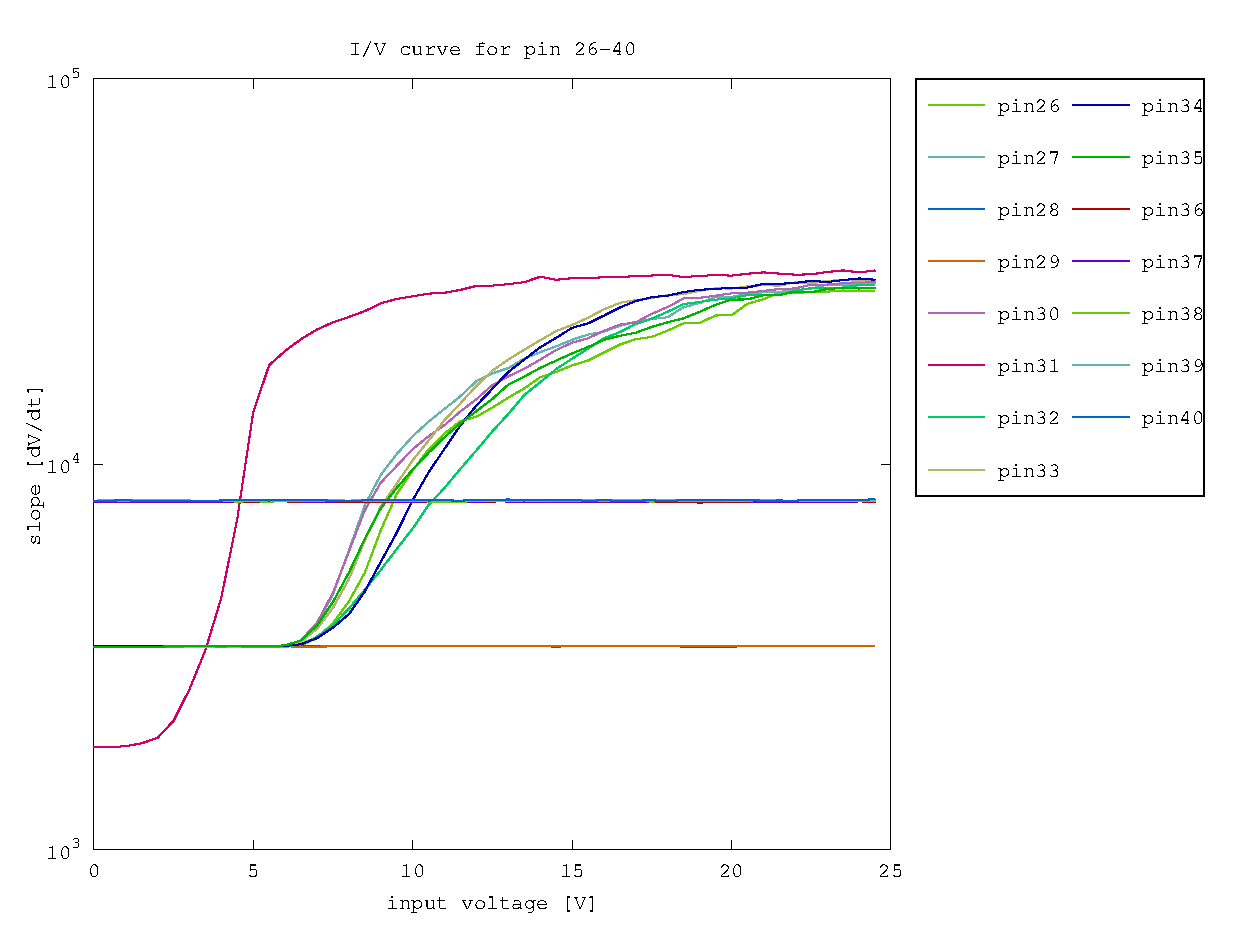
\includegraphics[width=\textwidth]{fig/pin26-40_slope_0-25V.eps}
	    \caption[Network2]%
	    {I/V characteristics}    
	    \label{fig:pin26-40_slope}
	\end{subfigure}
	\hfill
	\begin{subfigure}[b]{0.475\textwidth}  
	    \centering 
	    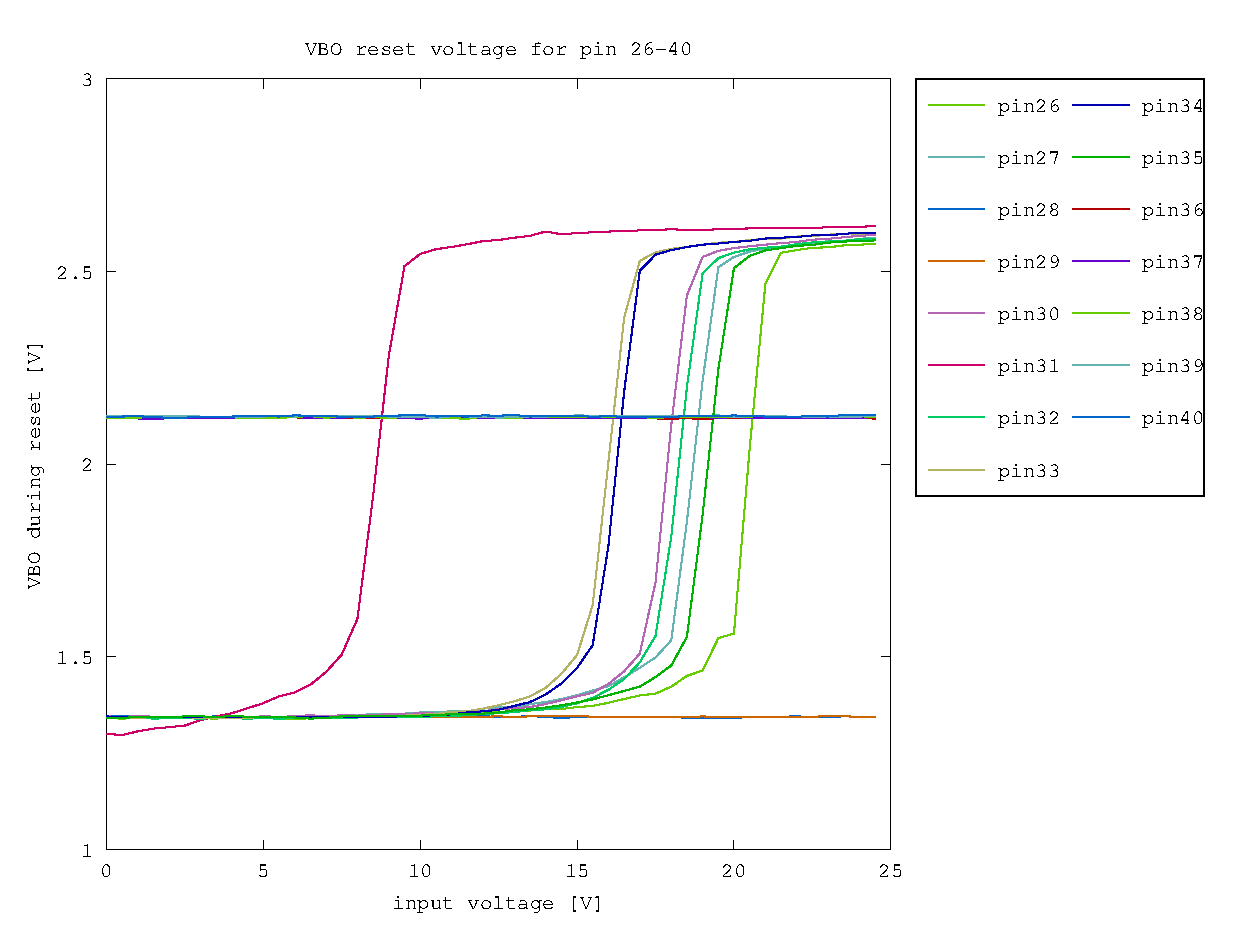
\includegraphics[width=\textwidth]{fig/pin26-40_reset_0-25V.eps}
	    \caption[]%
	    {reset value for VBO}    
	    \label{fig:pin26-40_reset}
	\end{subfigure}
	\caption{The slope and reset values for the VBO of pin26-40}
	\label{fig:pin26-40}
\end{figure}

\begin{figure}[h]
	\centering
	\begin{subfigure}[b]{0.475\textwidth}
	    \centering
	    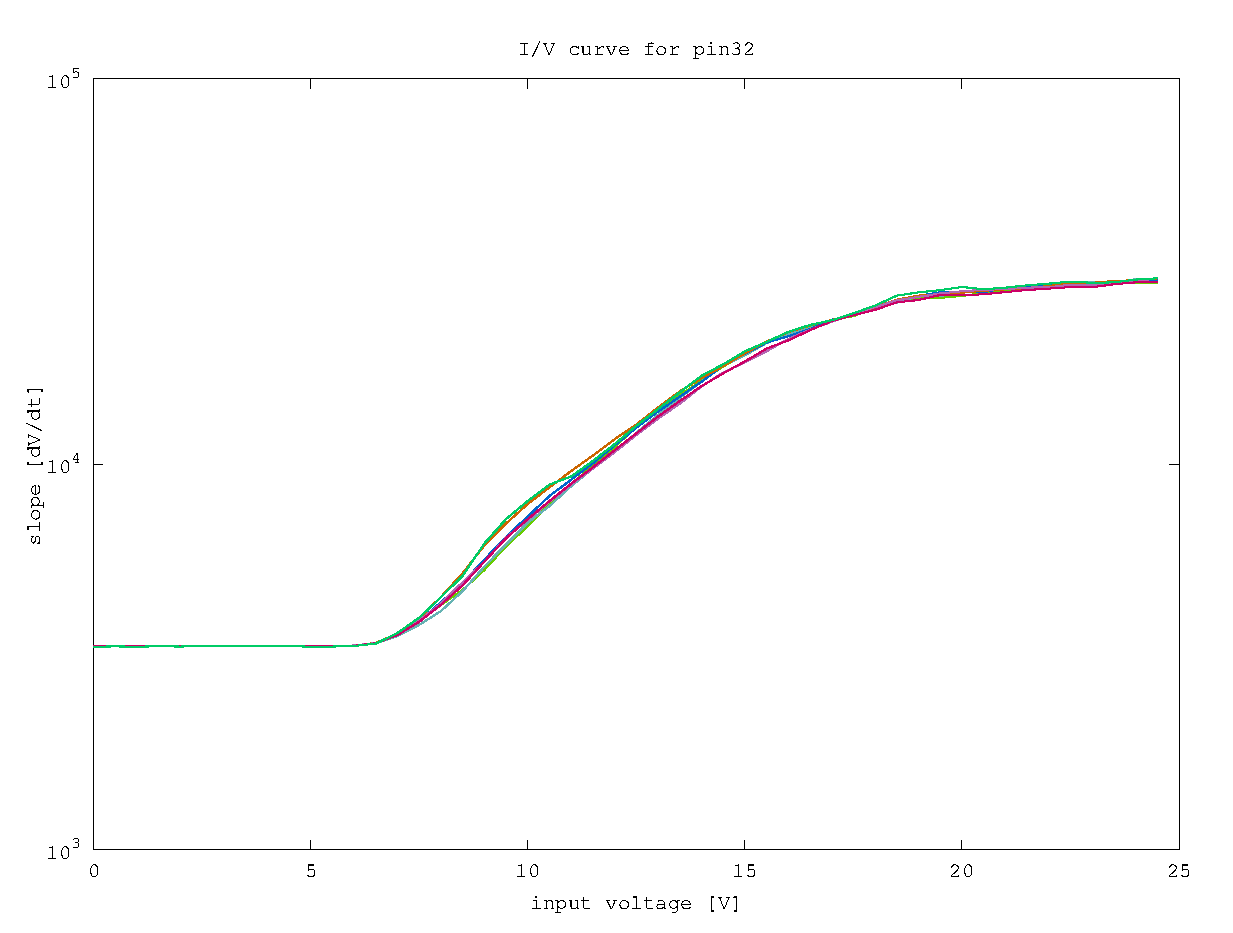
\includegraphics[width=\textwidth]{fig/pin32_slope_0-25V.eps}
	    \caption[Network2]%
	    {I/V characteristics}    
	    \label{fig:pin32_slope}
	\end{subfigure}
	\hfill
	\begin{subfigure}[b]{0.475\textwidth}  
	    \centering 
	    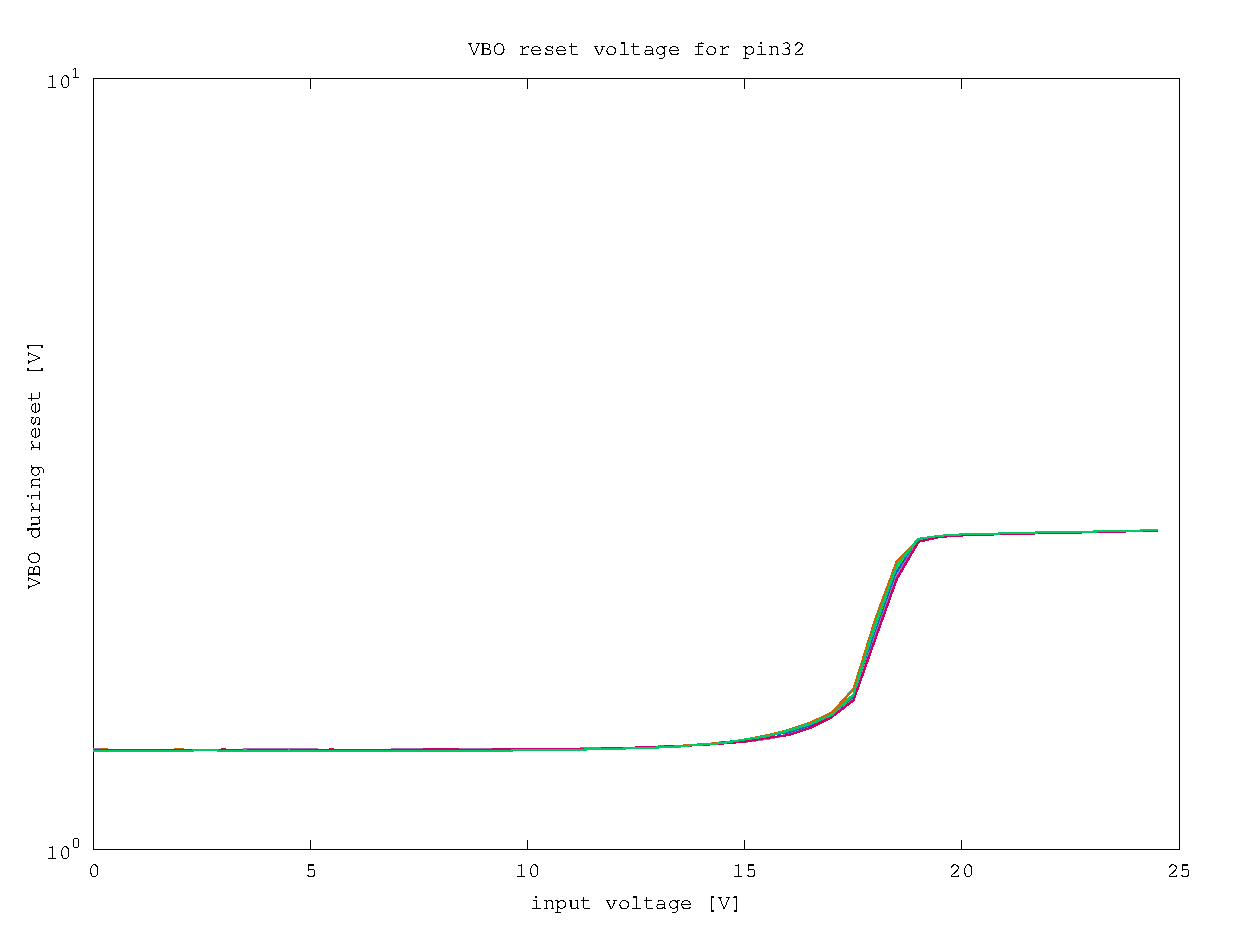
\includegraphics[width=\textwidth]{fig/pin32_reset_0-25V.eps}
	    \caption[]%
	    {reset value for VBO}    
	    \label{fig:pin32_reset}
	\end{subfigure}
	\caption{The slope and reset values for the VBO of pin32 repeated multiple times to test variance across measurements}
	\label{fig:pin32}
\end{figure}


The next step is to investigate reverse bias, and to achieve that the ground and pin input of the GaN sensor are switched around. The I/V characteristics for several pins are shown in \cref{fig:pin22_30_slope}. The jumps to negative current between 0 and $2.4\,V$ is due to the ROIC being $2.4\,V$. Therefore for lower voltages, the current flows into the opposite direction. The numbers are not representative for the actual current though, because the ROIC and measurement method are not designed for that direction of current. The main observation that can be made is that the voltage range available in the current setup is insufficient to observe the most intersting part of the I/V characteristics.  

\begin{figure}[h]
	    \centering
	    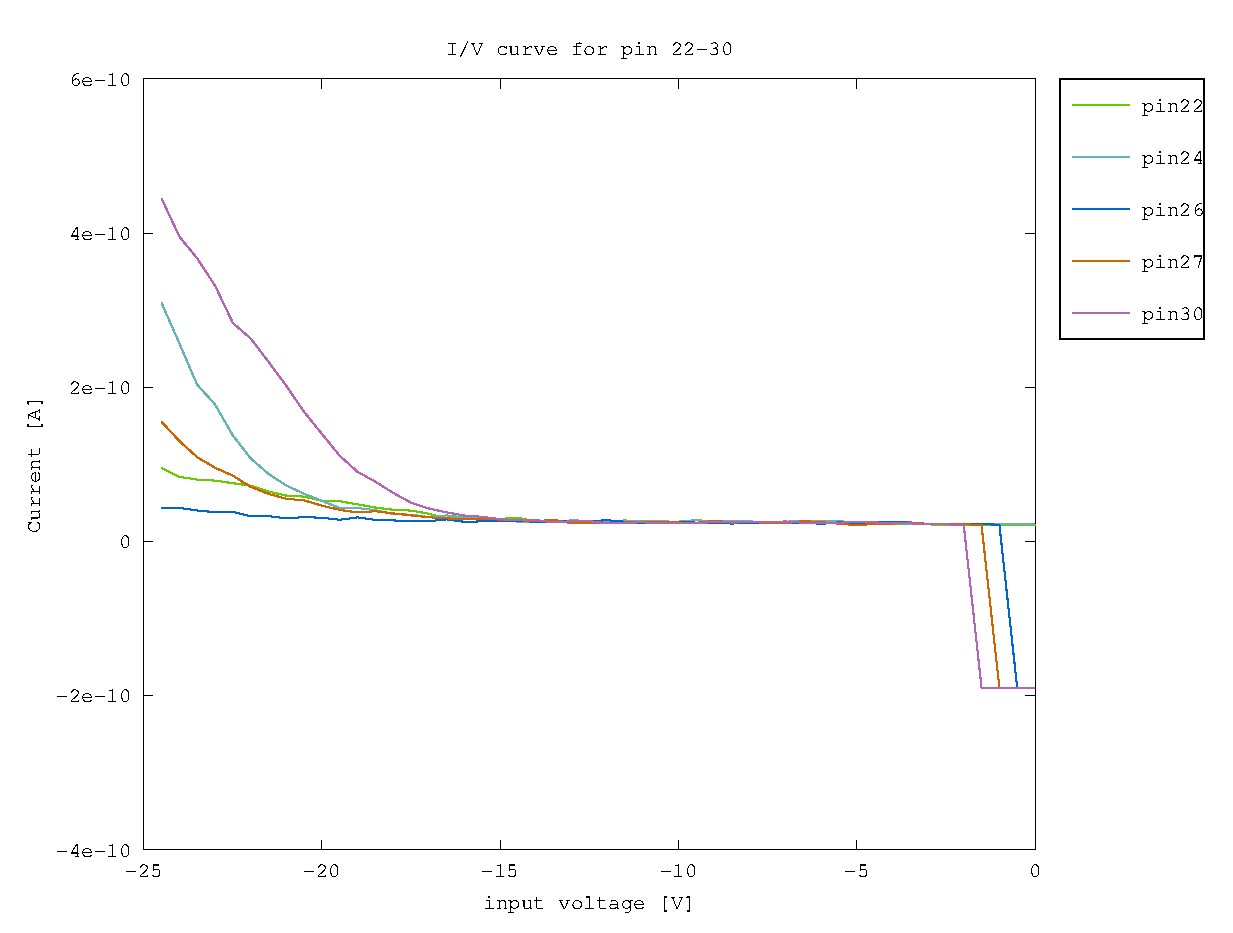
\includegraphics[width=\textwidth]{fig/pin22-30_slope_-25-0V.eps}
	    \caption[]%
	    {Voltage to current characteristics for several GaN sensors}    
	    \label{fig:pin22_30_slope}	
\end{figure}  


\subsection{High voltage range I/V characteristics}
In order to get a higher voltage range, tghe setup is changed again. The amplifier used for the input voltage caused a lot of noise and did not amplify enough. The new setup uses a manually controlled voltage source as input voltage. The input voltage is also measured by the oscilloscope. labVIEW continuesly takes measurements where it extracts both the current voltage and current. By manually sweeping the input voltage one can accumulate data points to construct the I/V characteristics. The I/V characteristics for pin 21 on the chip are shown in



\begin{figure}[h]
	    \centering
	    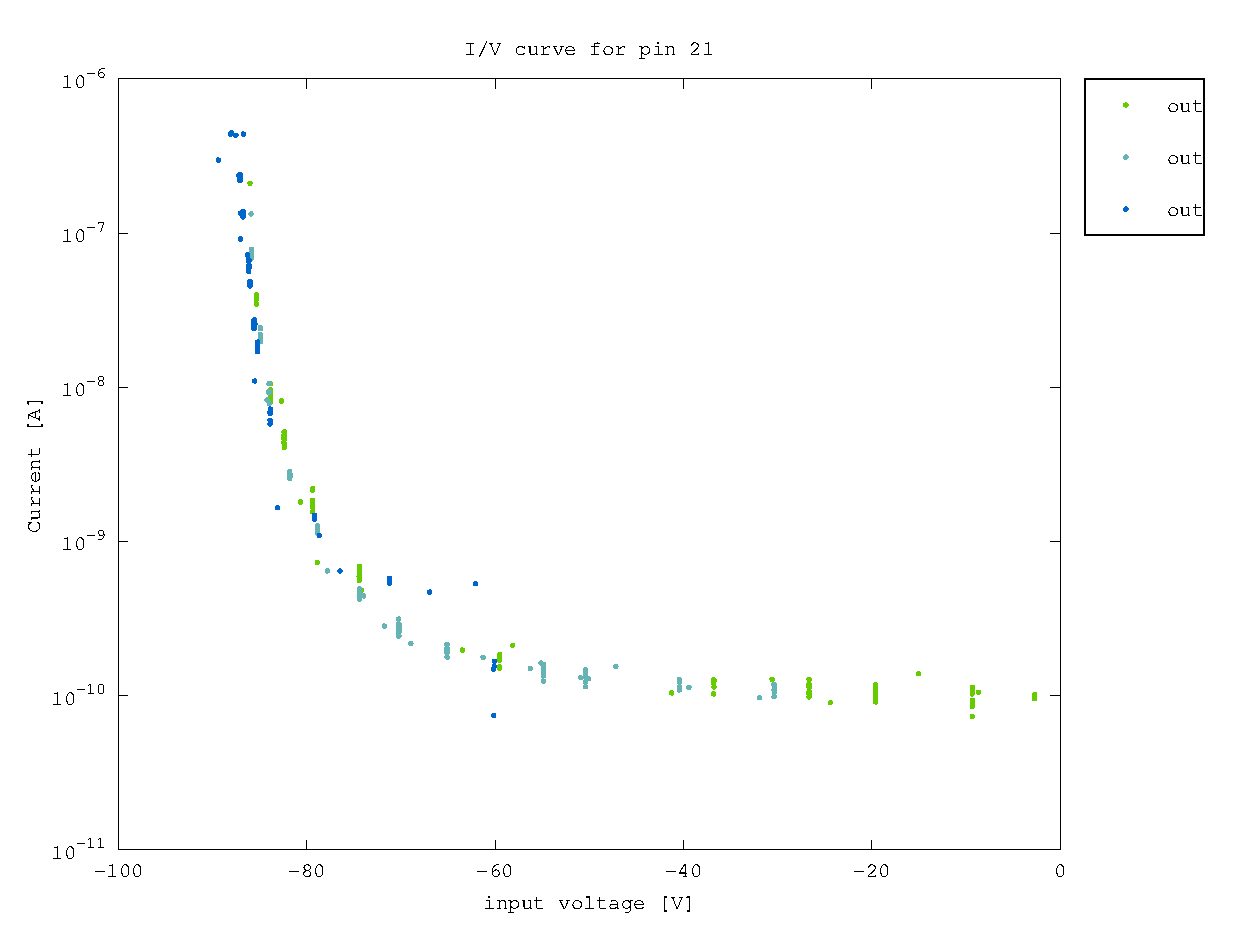
\includegraphics[width=\textwidth]{fig/pin21_slope.eps}
	    \caption[]%
	    {Voltage to current characteristics for several GaN sensors}    
	    \label{fig:pin22_30_slope}	
\end{figure}  

